\chapter{基于异构百科的跨语言属性对齐}
\label{cha:property-matching}

\section{本章引论}
本章从抽取更多跨语言知识,融合异构百科的角度出发,将工作定位于寻找百度百科与英文维基百科的中英文属性对齐关系。这是一个跨语言、跨异构百科的任务,就我们所知,当前还没有自动抽取百度百科属性信息,并与维基百科知识对齐的工作。

我们的工作面临跨语言与跨异构百科两项挑战,对于前者,因为维基百科与百度百科相互独立,在词条、分类乃至信息框属性方面,并没有直接的跨语言链接,如果能增加两者的关联信息,跨语言对齐的研究将会更加得心应手。得益于维基百科的多语言特性,我们可以通过中英文维基中已有的人工编辑的跨语言信息作为桥梁,连接英文维基与百度百科。

\section{问题描述}
本章的工作致力于解决中英文异构百科的跨语言信息框属性对齐问题。图\ref{fig:frozen-infobox}为电影《冰雪奇缘》在维基百科与百度百科中的信息框对比图,从左到右别为中文维基、英文维基、百度百科中的信息框。本章任务则是将指代同一个实体的中英文词条$a_e,a_z$中两个信息框中描述相同特性的属性对齐,比如\textit{Starring}对\textit{主演},\textit{Directed by}对\textit{导演}。

\begin{figure}[H]
  \centering
  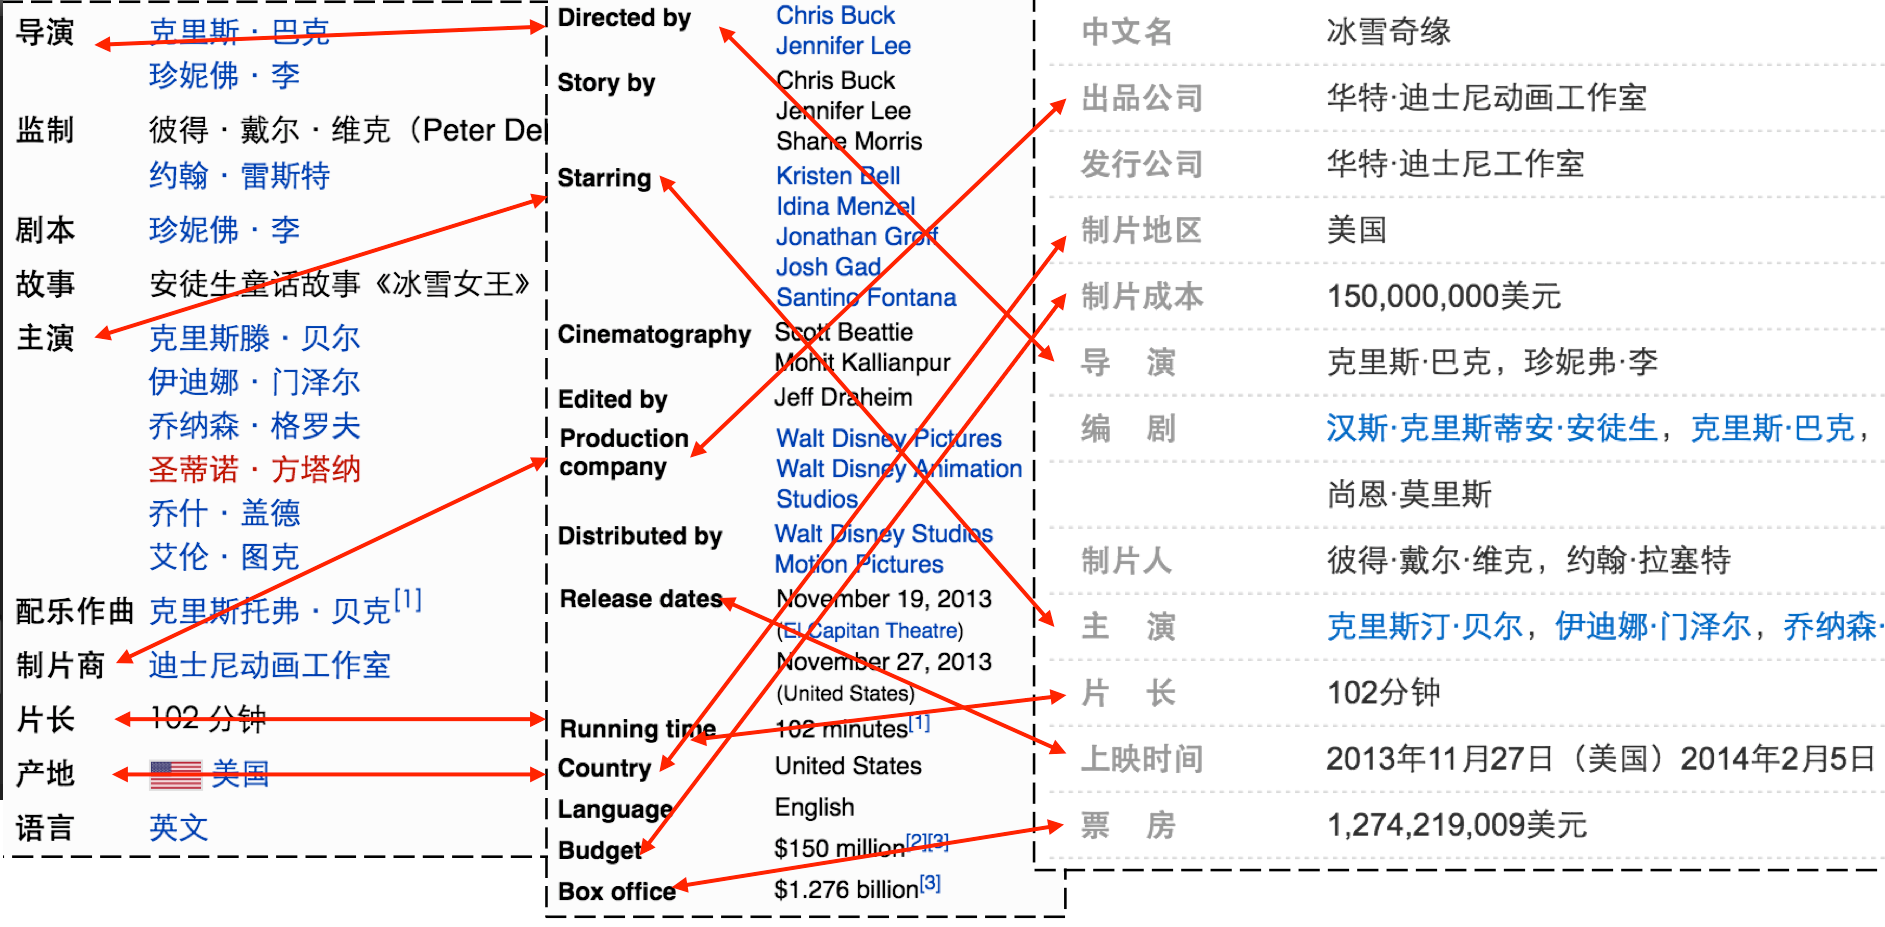
\includegraphics[width=0.9\columnwidth]{frozen-infobox}
  \caption{中英文信息框属性对齐示例}
  \label{fig:frozen-infobox}
\end{figure}

我们引入\ref{cha:concept-property}中的{\heiti 概念模板},认为属性在特定领域下的意思是唯一的。本文将对属性的分析限制在概念领域范围内,属性的同义词查找、跨语言链接等,都在同一领域里进行。为此,首先需要确定一个概念$c_i \in C$,并生成该概念下的属性集合(模板)$P(c_i)={p_1,...p_n}$。则本章问题可定义为:

给定对应的中英文领域$c_e \in C_E \leftrightarrow c_z \in C_Z$,找到其中的跨语言对齐属性对$p_{c_e} \leftrightarrow p_{c_z}$。

\section{异构百科的模板与属性分析}
\label{sec:template-property-analysis}

本章工作基于异构百科对齐中英文属性,除了跨语言的挑战,另一个挑战则是来自于维基百科与百度百科的异构性。

\subsection{词条数量不平衡}

维基百科是全球最大的百科数据库,目前支持228个语言。因语言使用者的差异、维基在各国的受欢迎程度等多种原因,英文维基词条与信息框数量远超其他语言,信息量很不对称。仅拿中英文来说,如图\ref{fig:en-zh-article-infobox-compare}所示,截止到2016年2月,英文维基词条约是中文维基的6倍,信息框差异更大,为是9倍。

\begin{figure}[H]
  \centering
  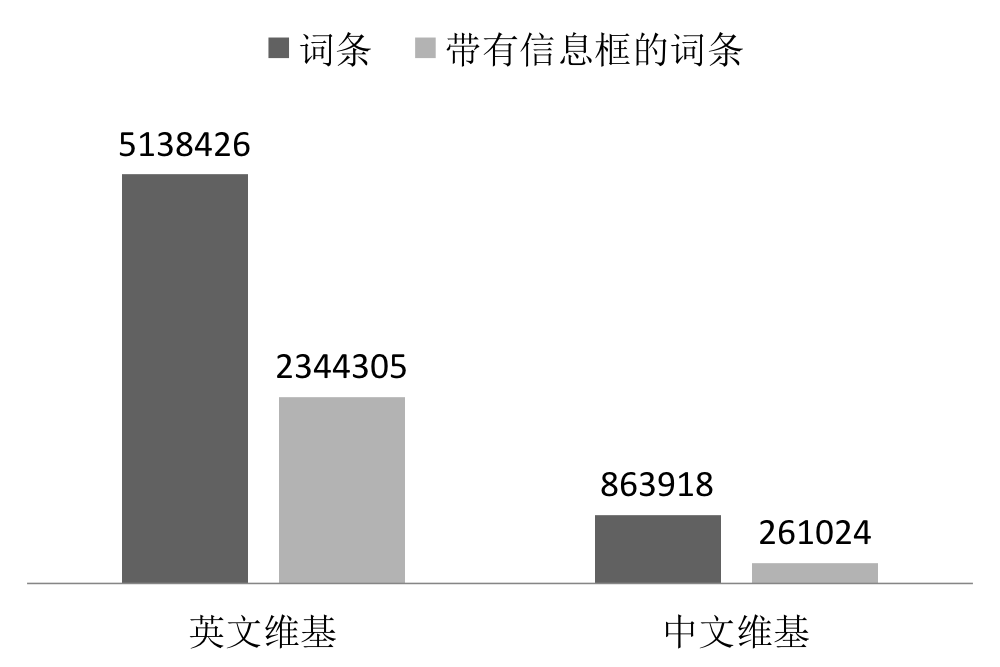
\includegraphics[width=0.6\columnwidth]{en-zh-article-infobox-compare}
  \caption{中英文百科词条数量对比}
  \label{fig:en-zh-article-infobox-compare}
\end{figure}

百度百科作为目前中国最大的开放式网络百科全书,收录了许多中国特色词条,因为参与编辑的人数多,编辑方式相对自由等原因,信息也更为全面。截止到2016年1月已收录词条超过1,313万条,远超过维基百科的中文词条数量。

图\ref{fig:frozen-infobox}表明三个百科中的信息各有异同,如果能充分利用三个百科之间的关系,比如通过百度百科的信息框补全中文维基信息框、利用中文维基与英文维基的对齐关系找到英文维基与百度百科的对齐关系等,就可以进一步促进知识补全,实现中英文知识融合。

\subsection{模板差异}

各个百科鼓励编辑者使用模板对词条进行组织与编辑。信息框的编辑也由模板来规范,比如百度百科中,描述人物使用\textit{人物通用模板},维基百科中,电影使用\textit{Template:电影信息框}。与此同时,用户在模板信息项之外,可自行添加自定义属性,丰富信息框内容,使其个性化。

利用模板信息,我们可以获得丰富的属性集合以及属性与概念领域的对照关系。理想情况下,只要能找到跨语言下的异构百科中模板的对应关系,就能获得相关的属性的对齐关系,达到跨语言、跨领域属性对齐的目标。但是实际上,这个过程存在诸多阻碍:
\begin{itemize}
\item 百度百科模板无法获取。百度百科数据用于商业用途,没有像维基百科一样公开数据,因此百度百科数据的获取多来源于网络爬虫。虽然网页涵盖了词条的几乎所有内容,但并不包含编辑信息,比如模板的使用。因此我们只能获得百度百科的属性集合,并依赖进一步的研究方法,猜测模板内容。
\item 异构百科定义的模式不同。姑且不说中英文差异,单是中文维基与百度百科,在对同一概念下词条的描述,命名规范与侧重点都不尽相同。以完成度较高的电影领域模板为例,\ref{fig:frozen-infobox}中可以看到,中文维基使用\textit{制片商},百度百科使用\textit{出品公司}作为电影制作公司属性的标签,可见{\heiti 属性多义性}。另一方面中文维基常有\textit{旁白}、\textit{配乐作品}等百度百科不使用的属性,百度百科常有\textit{imdb编码}等维基模板中没有的属性,可见{\heiti 模板缺失性}。若想尽可能保留属性集合的完整度,保证准确度,我们需要处理属性多义与模板缺失问题。
\end{itemize}

模板的差异,无论是对前期的属性抽取,还是对之后的属性对齐工作,都带来了更多的挑战,但这也表明异构百科下属性的使用,确实有值得探究之处。我们可以通过寻找同一种属性在异构百科下的不同表达方式,寻找相似属性名称;融合多个百科的属性集合,获得领域下更全面的属性集合,制成通用模板。

\section{基于异构百科的跨语言属性对齐}
\label{sec:property-matching}

本章致力于解决跨语言概念属性的对齐,由于数据的不规范,我们需要解决百度百科概念属性生成、同义属性合并等诸多问题。

%本任务获得的领域下的属性模板,可以避免人工构建模板,有助于增加信息框的有意信息,查漏补缺,另一方面,获得属性同义表达方式,可以为融合其他百科信息做铺垫。属性模板的构成、属性的分布、属性的命名,在一定程度上都可以对用户行为分析、文本分析做贡献。比如一个实体的关键信息都有什么、用户一般关注什么重点信息、人们多属性的常用称呼都有什么等等。一旦拥有属性模板,我们可以用自动化的方法,从文本中抽取相应的信息,自动构建词条信息框。[引用][][]中都在已知属性集合的基础上,对缺失属性进行填充。

图\ref{fig:property-matching}为整个跨语言属性对齐的框架图,根据前文所提出的问题,主要分为概念属性生成、同语言属性对齐与相似属性合并、跨语言种子集合生成、跨语言属性对齐四大模块。

\begin{figure}[H]
  \centering
  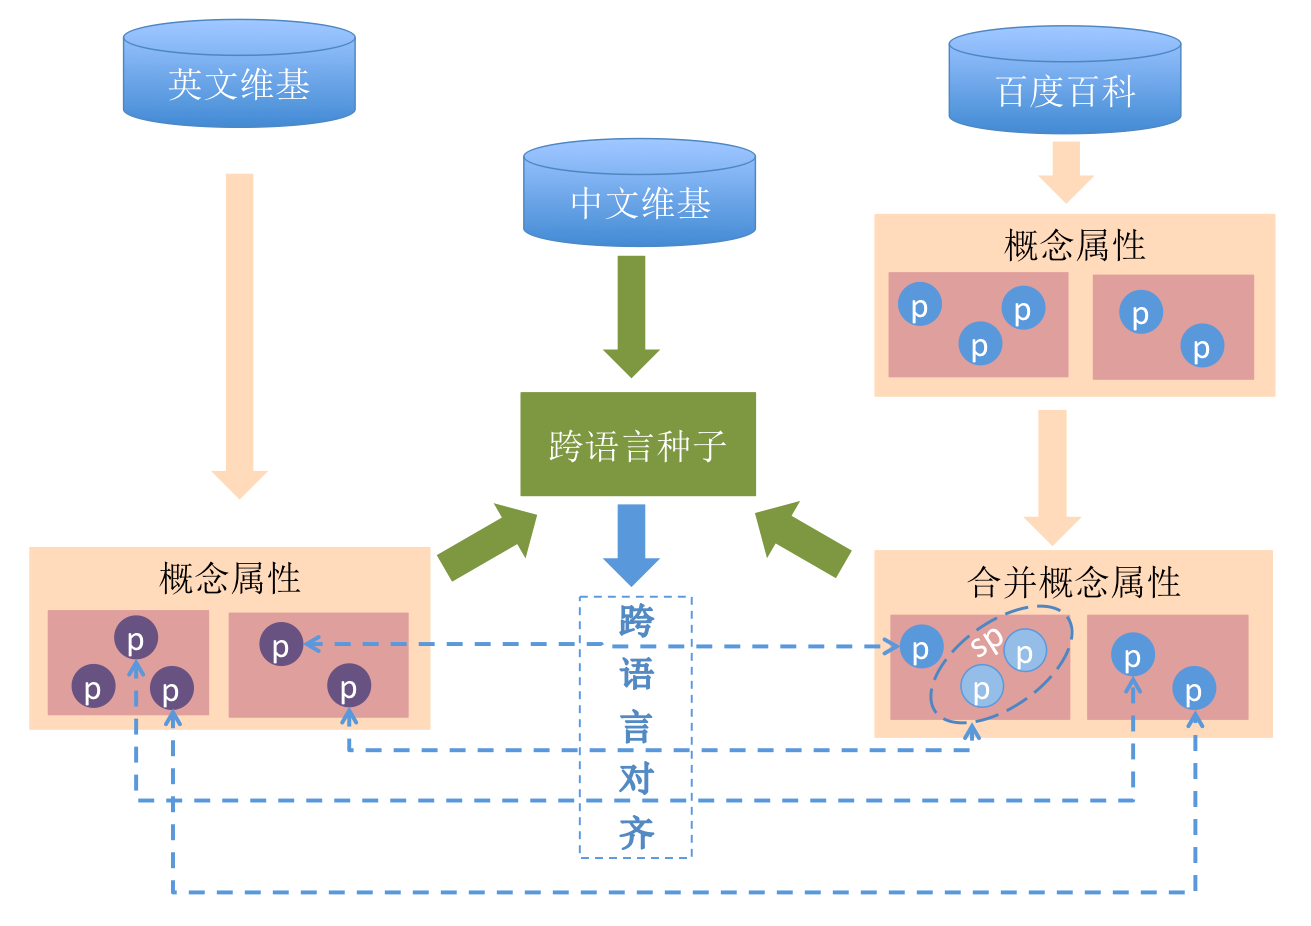
\includegraphics[width=0.8\columnwidth]{property-matching}
  \caption{跨语言属性对齐框架图}
  \label{fig:property-matching}
\end{figure}

本章数据基于\ref{cha:concept-property}中的结果数据,以及从2014年12月版本的百度百科网页上获取的信息。不同于维基百科复杂的概念属性抽取,百度百科页面不含模板信息,通过网页解析即可获得结构化信息,在此不做赘述。

{\heiti 百度百科概念模板生成:}针对百度百科没有信息框模板这一问题,我们根据属性词频与共现率,提出概念属性生成模型,旨在对给出的维基概念,在百度百科数据中模拟出对应的概念与概念属性集合,进而形成模板。概念属性集合,可作为今后编写信息框的参照,同时可看作属性对齐的候选集,大大减小了计算空间。

{\heiti 同语言属性对齐与相似属性合并:}针对属性的一义多词问题,即描述相同意义的属性,有不同的显示标签。
%我们从文本相似度、语义形似度等角度出发,计算获得特定属性的同义属性。
我们通过对齐中文维基与百度百科属性,找出高质量的属性同义词,这对提高跨语言对齐的召回率有帮助。

{\heiti 跨语言种子集合:}维基百科与百度百科这两个异构百科没有直接的关联关系,但以中文维基为桥梁,并利用维基的跨语言特性,我们找到百度百科与中英文维基百科的联系,抽取出一部分高准确度的属性对齐关系。
%信息框属性在维基百科中,不像分类与词条一样含有显性的语言链接,不能直接获取,但我们依然可以通过信息框模板与词条链接等现有关系,抽取出正确的属性跨语言对齐关系。
%另一方面,通过分析同语言百科,获得对齐的中文属性集合。两两融合后,获得英文维基-中文维基-百度百科的属性对齐关系,形成跨语言种子集合。

{\heiti 跨语言属性对齐:}种子集合只包含小部分常用且识别度高的属性对齐关系,对于剩下的长尾问题,我们训练一个二元分类器,判断给定的中英文属性对是否为对齐关系。其中特征主要从文本、结构中抽取。

\subsection{百度百科概念模板生成}
\label{sec:domain-template}
根据模板的定义,我们提出如下假设:给定一个概念领域,在其中使用频率高,或在其他领域极少出现的属性,即为该领域的属性。该思想与TF-IDF(term frequency–inverse document frequency)的思想相近,TF-IDF表征一个词在一类文档中的重要程度,可以用来区分不相关文档。属性在领域的IF-IDF值,可以表示该属性对领域的相关程度。

如何圈定一个概念及其相关信息?在\ref{cha:concept-property}中,我们认为模板规范着一类文档的写作,关联着一个概念领域,即$T \approx C$。\ref{cha:concept-property}中抽取的信息框模板覆盖了90\%的维基文档,可以认为涵盖了百科中的大部分领域。由于英文维基的模板已知,当前的任务可以定义为:给定概念$C_E$,在百度百科$W_b$中抽象出与其对应的中文概念$C_Z$,及其属性集合$P(C_Z)={p_1^z,...,p_n^z}$。其中,不同于$C_E$有明确的模板定义,$W_b$中的$C_Z$是一个抽象存在,可以认为$P(C_Z)$就代表着$C_Z$中实例的特性,$P(C_Z)$组成概念领域$C_Z$的模板。

哪些属性可以涵盖在$C_Z$内?我们首先获取$P(C_Z)$的候选集。根据百科的结构,可以通过直接关联找到关系密切的属性,并利用间接关系扩展属性候选:

{\heiti 直接关联} $C_E$中的词条$A(C_E)$对应的跨语言词条集合$A_Z$使用的属性,认为是与$C_E$直接关联的属性,定义为$p_direct$;

{\heiti 间接关联} $C_E$中的词条$A(C_E)$涉及的分类$Ca(C_E)$对应的跨语言分类集合$Ca_Z$下,对应词条$A_Z'$使用的属性,认为是与$C_E$间接关联的属性,定义为$p_indirect$

则有:
\begin{align}
\label{equ:tf}
tf_{i,j}=\frac{n_{i,j}}{\sum_{k}{n_{k,j}}}
\end{align}
\begin{align}
\label{equ:idf}
idf_{i}=1+log\frac{\left | D \right |}{\left | j:t_i  \epsilon d_j \right |}
\end{align}
\begin{align}
\label{equ:tfidf}
ifidf_{i,j}=tf_{i,j}\times idf_{i}
\end{align}

\ref{equ:tf}中$n_{i,j}$是属性在领域$d_{j}$中的使用频次,分母则是在领域$d_{j}$中全部属性的使用次数之和。对属性频次的计算,因为直接关联属性比间接关联属性更重要,权值应更高,因此

\begin{align}
n_{i,j} = {\sum_{k}{x_{k,j}}}\\
\end{align}

\begin{align}
x_{k,j} =
\left\{\begin{matrix}
2 & p_i = p_{direct} \ in \ d_j\\
1 & p_i = p_{indirect} \ in \ d_j\\
0 & p_i \ not \ in \ d_j
\end{matrix}\right.
\end{align}

\subsubsection{结果}
\ref{tab:baidu-template-examples}给出两个典型概念下属性集合:

\begin{table}[htb]
  \centering
  \caption{百度百科概念模板生成结果举例(前20)}
  \label{tab:baidu-template-examples}
    \begin{tabular}{cccc}
      \toprule[1.5pt]
         \multicolumn{2}{c}{Planet} & \multicolumn{2}{c}{电影信息框}\\ \midrule[1pt]
         发现者   &  自转周期  & 导演     & 其他译名 \\
         发现时间 &  离心率    & 制片地区 & 外文名   \\
         中文名   &  绝对星等  & 片长     & 出品时间 \\
         质量     &  反照率    & 主演     & 出品公司 \\
         公转周期 &  平近点角  & 上映时间 & imdb编码 \\
         分类     &  别称      & 对白语言 & 制片人   \\
         直径     &  半长轴    & 类型     & 分级     \\
         外文名   &  平均密度  & 编剧     & 发行公司 \\
         发现日期 &  表面温度  & 色彩     & 拍摄日期 \\
         倾倒斜角 &  天体名称  & 中文名   & 拍摄地点 \\
      \bottomrule[1.5pt]
    \end{tabular}
\end{table}


\subsection{同语言对齐与相似属性合并}
\label{sec:similar-property}

{\heiti 中文维基与百度百科属性对齐}是在同语言环境下,找出中文属性对齐关系。为获取更多异构百科中的跨语言对齐关系做准备。具体来说:

\begin{enumerate}[1)]
\item {\heiti 基于属性名称:}   描述同一实体的两个百科词条中,如果信息框属性名称一致,认为是同一属性;
\item {\heiti 基于相同属性值:} 描述同一实体的两个百科词条中,如果信息框属性名称有相同字符,且属性值相同,则认为是同一属性;
\item {\heiti 基于相似属性值:} 描述同一实体的两个百科词条中,如果信息框属性属性值相似,则认为是同一属性。为保证准确性,我们添加置信度衡量标准,即相似出现频率超过$N$次($N=5$)。
\end{enumerate}

因为个人编写习惯,百科监管不严格等问题,属性可能有多种表达方式。我们在对齐结果中,发现中文维基一个属性可能对应多个百度属性标签,比如电影概念下,\textit{剪辑}有\textit{剪辑},\textit{剪辑导演},\textit{剪接}等表示方法,验证了这一现象的普遍性。

如果一个属性有多个表示方法,应该将其视为一个属性。我们将代表同样含义但不同标签的属性合并成一个超属性$sp=\{p_1,...,p_n\}$。百度百科的每个属性都由$sp$来表示,如果某属性没有歧义表达,则$sp={p}, \ {\#sp}=1$。

本节中的同语言对齐方法较为严格,准确率较高,其一对多的情景抽象出的$sp$可以直接利用。因为对齐结果较少,我们对其进行了人工验证,准确率在。。。

为寻找更多的相似属性,还可以进一步通过文本、值域、结构等维度入手,对属性聚类。在理想情况下,一个簇表示一个超级属性。

我们尝试从文本相似度、Word2Vec语义相似度,值相似度三个维度特征入手,对百度百科同一领域的属性进行聚类。以\textit{电影(film)},\textit{公司(company)}, textit{歌曲(single)}三个领域的结果进行检查,并与对齐方法进行对比,见表\ref{tab:similar-property-compare}

\begin{table}[htb]
  \centering
  \caption{方法对比结果}
  \label{tab:similar-property-compare}
    \begin{tabular}{ccccc}
    \toprule[1.5pt]
      {\heiti 方法} & {\heiti 准确率} & {\heiti 召回率} & {\heiti 相似属性数量} & {\heiti 超属性数量(${\#sp}>1$)} \\\midrule[1pt]
      基于同语言对齐 & 1 & 1 & 1 & 1 \\
      聚类方法       & 1 & 1 & 1 & 1 \\
      \bottomrule[1.5pt]
    \end{tabular}
\end{table}

经过表\ref{tab:similar-property-compare}中对比可看出,基于聚类方法的同语言对齐,虽然在对齐数量上有明显增加,提高了召回率,但准确率却有所损失。超属性作为之后跨语言对齐的对象,其存在的瑕疵会造成错误累加,因此对其质量要求很高。基于此,我们使用同语言对齐时获得的相似属性结果,以保证之后工作的高质量。

\subsection{跨语言属性种子集合生成}
\label{sec:cross-lingual-seed}
依赖维基百科跨语言特性,我们首先可以获得一批高质量的中英文属性对齐关系,以此为媒介,进一步寻找维基与百度百科的属性对齐关系。该过程可分为三个子步骤,即分别构建中英文维基百科、中文维基与百度百科、英文维基与百度百科的属性对齐关系。

{\heiti 第一步 中英文维基百科跨语言属性对齐}在维基的语言链接,即现有跨语言模板与跨语言词条基础上实现。具体来说,分为三种情况,图\ref{fig:cross-lingual-seed}给出了较为直观的展示:

\begin{figure}[h]
%  \centering%
%  \begin{subfigure}{0.48\textwidth}
%    \centering
%    
\includegraphics[width=0.8\textwidth]{enwiki-zhwiki-property-crosslinks-1}
%    \caption{基于跨语言模板对齐}
%  \end{subfigure}%
%  \hspace{0.01cm}%
%  \begin{subfigure}{0.48\textwidth}
%    \centering
%    
\includegraphics[width=0.8\textwidth]{enwiki-zhwiki-property-crosslinks-1}%为了对齐和上面用的同一张图
%    \caption{基于跨语言实例对齐}
%  \end{subfigure}
%  \vspace{0.01cm}%
%  \begin{subfigure}{0.5\textwidth}
%    \centering
%    
\includegraphics[width=0.8\textwidth]{enwiki-zhwiki-property-crosslinks-3}
%    \caption{基于属性值对齐}
  %\end{subfigure}
  \centering
    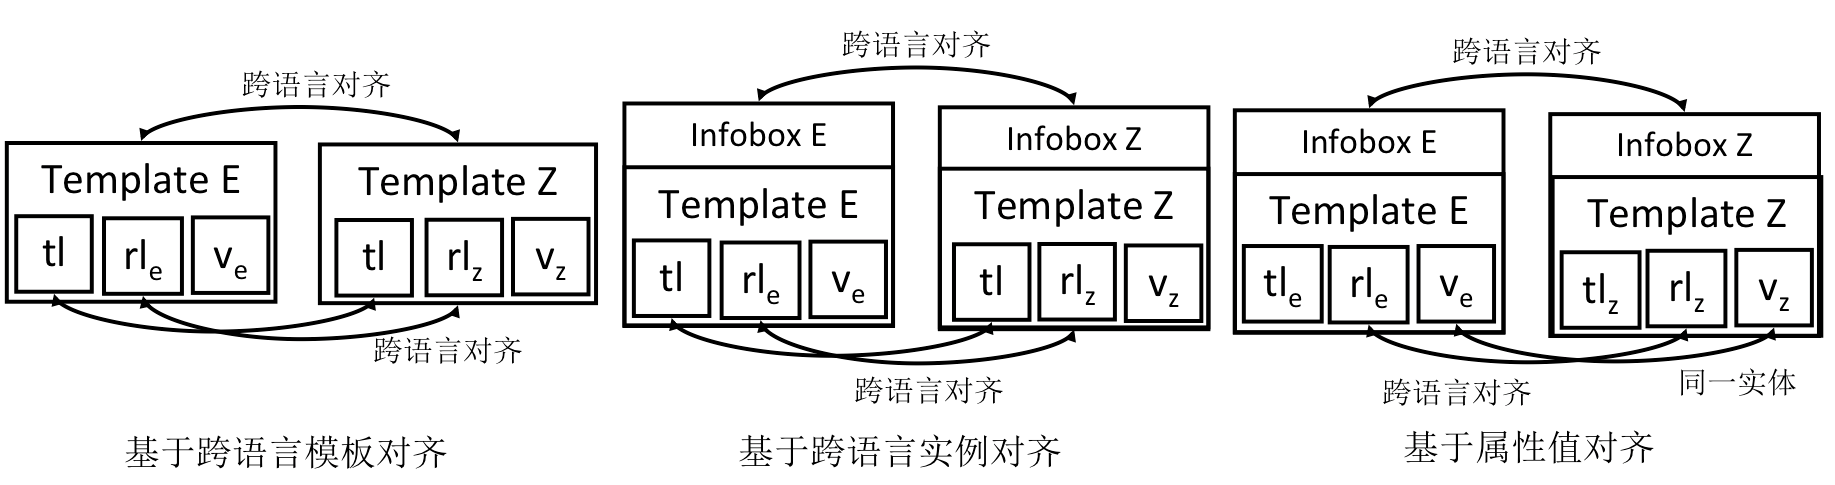
\includegraphics[height=4cm]{cross-lingual-seed}
  \caption{中英文维基属性跨语言抽取说明}
  \label{fig:cross-lingual-seed}
\end{figure}

\begin{enumerate}[1)]
\item  {\heiti 基于跨语言模版对齐:}对于已对齐的跨语言信息框模版$<T_e, T_z>$,找出模板标签一致的中英文显示标签,构成跨语言属性对,即如果$p_e(T_e).tl_e == p_z(T_z).tl_z$,则$<p_e(T_e), p_z(T_z)>$是跨语言链接对;
\item  {\heiti 基于跨语言实例对齐:}对于已对齐的词条$<a_e, a_z>$,抽取其信息框模版$<T_e'(a_e), T_z'(a_z)>$,找出其中模板标签一致的中英文显示标签,构成跨语言属性对,即如果$p_e(T_e').tl_e == p_z(T_z').tl_z$,则$<p_e(T_e'), p_z(T_z')>$是跨语言链接对;
\item  {\heiti 基于属性值对齐:}对于已对齐的词条$<a_e, a_z>$,分析其信息框中的属性-属性值,如果两个中英文属性类型都为对象属性,且属性值指向同一个实体;这两个属性构成跨语言属性对,即如果$p_e(a_e).v and p_z(a_z).v are entities$ 且 $<p_e(a_e).v, p_z(a_z).v>$是跨语言对齐的关系,则$<p_e(a_e), p_z(a_z)>$是属性跨语言链接对。
\end{enumerate}

{\heiti 第三步 跨语言种子集合生成},即英文维基与百度百科属性对齐结果,利用前两步的结果作为媒介,两两对齐,获得双语对齐关系。

\subsubsection{实验结果}
在第一步中,我们从2016.02版的中文维基与2016.03版的英文维基中获取中英文对齐关系。表\ref{tab:zhwiki-enwiki-cross-lingual}中统计了三种方法分别获得的跨语言属性链接数量,并举出例子。

\begin{table}[htb]
  \centering
  \caption{中英文维基属性跨语言对齐结果}
  \label{tab:zhwiki-enwiki-cross-lingual}
    \begin{tabular}{ccc} 
      \toprule[1.5pt]
      {\heiti 对齐方法} & {\heiti 数量} &  {\heiti 举例} \\\midrule[1pt]
      基于跨语言模板对齐 & 16104 & Editing by  剪辑 Date(s) 日期   \\
      基于跨语言实例对齐 & 124 & 1  memory 记忆体 manufacturer [[制造商]]\\
      基于属性值对齐     & 129 & associated acts 相关团体 num episodes 集数  \\
      总数               & 16357 & -  \\
      \bottomrule[1.5pt]
    \end{tabular}
\end{table}

第二步我们使用2014.12版本的百科数据与中文维基进行对齐。经历三步提取,最终结果在表\ref{tab:zhwiki-baidu-cross-lingual}中展示。

\begin{table}[htb]
  \centering
  \caption{中文维基与百度百科属性对齐结果}
  \label{tab:zhwiki-baidu-cross-lingual}
    \begin{tabular}{ccc}\toprule[1.5pt]
      {\heiti 对齐方法} & {\heiti 数量} &  {\heiti 举例} \\\midrule[1pt]
      基于属性名称   & 2324 & Template:Infobox Game   [[游戏发行商|发行商]]   发行商  \\
      基于相同属性值 & 2365 & Template:Infobox Game   适用年龄    年龄 \\
      基于相似属性值 & 3781 & Template:Infobox scientist  获奖    主要成就  \\
      总数           & 8470 & -  \\
      \bottomrule[1.5pt]
    \end{tabular}
\end{table}

在最终的跨语言属性种子集合生成结果中,我们以{\heiti 模板:属性标签}表征一个属性,即属性带有概念信息。
%我们还发现,对于一个属性,可能有一义多词的现象出现。
最终结果统计见表\ref{tab:cross-lingual-seed},表\ref{tab:cross-lingual-seed-examples}给出了对齐示例。

\begin{table}[htb]
  \centering
  \caption{跨语言属性对齐种子集合结果}
  \label{tab:cross-lingual-seed}
    \begin{tabular}{ccc}\toprule[1.5pt]
      {\heiti 对齐数量} & {\heiti 概念数量} \\\midrule[1pt]
      2262 & 235  \\
      \bottomrule[1.5pt]
    \end{tabular}
\end{table}

\begin{table}[htb]
  \centering
  \caption{跨语言属性对齐种子举例}
  \label{tab:cross-lingual-seed-examples}
    \begin{tabular}{ccc}\toprule[1.5pt]
      {\heiti 概念} & {\heiti 英文属性} &  {\heiti 中文属性} \\\midrule[1pt]
      \multirow{5}{*}{电影} 
      & Box office    & 累计票房/全球票房/票房  \\
      & Budget        & 制片成本/预算/电影投资  \\
      & Directed by   & 导演/编剧  \\
      & Distributed by & 出品公司/发行商/发行方/发行公司  \\
      & Release dates & 上映日期/上映/首映日期/上映时间/播放期间  \\ 
      \midrule[1.0pt]
      \multirow{5}{*}{大学} 
      & Active       & 创建时间/建立时间/创办时间/办学时间  \\
      & Affiliations & 主管部门  \\
      & Former names & 老校名  \\
      & Location     & 所属地区/地址/校址/学校地址  \\
      & President    & 院长/董事长/现任校长/现任院长 \\
      \bottomrule[1.5pt]
    \end{tabular}
\end{table}

\subsection{跨语言属性对齐}
\label{sec:cross-lingual-property-matching}
对齐是一对一匹配的精准工作,为了让结果可精确且可度量,我们将跨语言属性对齐设计成二分类任务,即“对齐”返回1,“非对齐”返回0,并采用逻辑斯谛回归模型进行训练与预测。

\subsubsection{特征选择}
特征选用三类特征:基于文本特征、基于结构特征、基于分布特征。

{\heiti 基于文本特征} 我们对两部分文本进行计算,分别为属性标签和属性值。针对语言的差异,我们利用百度翻译API\footnote{http://fanyi.baidu.com/},获得属性标签中译英、英译中两类翻译结果,与属性值英译中翻译结果。文本相似度多采用编辑距离(EditDistance)计算,编辑距离相似度被定义为:
\begin{equation}
ed\_sim(s_1, s_2) = \frac{edit\_distance(s_1, s_2))}{max(\left| s_1 \right |,\left | s_2 \right |))}
\end{equation}

标签相似度:对中英文属性的标签进行计算,转换成同语言后,分别进行中文相似度计算与英文相似度计算,取最大值作为特征值。
\begin{equation}
\label{}
sim_{label}(sp_e, sp_z) = max(ed\_sim(label(p_e), label'(p_z)), ed\_sim(label'(p_e), label'(p_z)))
\end{equation}
其中$label'$为属性标签对应的翻译字符串。

属性值相似度:属性值是衡量两个属性是否对齐的最直接指标,如果两个属性在同一篇词条下具有相同属性值,它们匹配的可能性就很大。根据属性值的内容,我们将其分为三类,分别为文章型、数字型、纯文本型,每一种类型,采用不同的相似度计算策略。

文章型属性值:如果属性值表示一个实体,即其链接到一个词条,认为它是文章型属性。这类属性,对于其“相等”的定义为:如果两个实体是跨语言链接关系,即表征同一实体,则认为属性值相等:
\begin{equation}
Equal(a,a')=\left\{\begin{matrix}
1 \ if <a,a'> in \ CL\\
0 \ else
\end{matrix}\right.
\end{equation}

文章型属性的相似度计算公式如\ref{equ:article_value_similarity}:

\begin{equation}
\label{equ:article_value_similarity}
sim_{article\_v}(sp_e, sp_z) = \frac{\sum_{a_e\in A(sp_e), a_z \in A(sp_z)} Equal(a_e, a_z)}{min(\left| A(sp_e)\cap CL(A_E) \right|, \left|A(sp_z) \cap CL(A_Z) \right|)}
\end{equation}
$A(sp)\cap CL(A)$为含有跨语言链接的词条集合。

数字型属性值:由数字构成的值,比如年龄、日期、电影票房等,被定义为数字型属性值。对于这类属性值,不能直接对比,也不适合用文本相似度计算方法。我们还面临异构百科带来的另一个问题:不同百科中,同一属性的属性值可能由不同形式表示,比如迈克尔·菲尔普斯(Michael Phelps)在英文维基中,身高(Height)为“6 feet 4 inches”,而在百度百科中则表示成193cm。考虑到以上特点,我们用皮尔逊积矩相关系数(Pearson product-moment correlation coefficient)计算数字型属性值的相似度,该系数衡量两个变量的线性相关程度。具体见公式\ref{equ:number_value_similarity}

\begin{equation}
\label{equ:number_value_similarity}
sim_{number\_v}(sp_e, sp_z) =
\end{equation}

文本型属性值:既不指向实体,又没有数字特征的属性值,被认为是文本型属性值。我们用编辑距离方法计算其相似度\ref{}:

\begin{equation}
\label{equ:literal_value_similarity}
sim_{literal\_v}(sp_e, sp_z) =
\end{equation}

为了减小计算复杂度并提高准确度,属性值最好在精炼且可能性大的候选集中计算。因此我们将属性值相似度的计算粒度设定为单个文章,即只与对齐文章信息框内的属性值进行比对。

%\begin{equation}
%\end{equation}

{\heiti 基于结构特征}
当前大部分跨领域的知识库都以在线百科为数据源而建立。百科内部本身就存在着一些语义关系,比如子分类和父分类间的\textit{subClassOf}关系、词条实体与分类之间的\textit{instanceOf}关系。语义信息常被用来抽取特征\cite{wang2014cross},表示实例等在结构上的特点。我们利用百科里现有的语义关系,抽取出两个特征,分别为文章相似度与概念相似度。

文章相似度即计算使用两属性词条的交集,定义为:\ref{},概念相似度即计算两属性领域的相似程度。

%基于语义的特征表征的是两个
{\heiti 基于分布特征}
是基于假设:\textit{同一属性即使在不同百科中,被使用频率也相近。}我们称之为受欢迎(Popular)程度,该特征的定义为:
\begin{equation}
sim_{popular}(sp_e, sp_z) =
\end{equation}

\subsubsection{实验结果}

{\heiti 评测标准}
作为标准的二分类模型,我们用准确率(Precision),召回率(Recall),与F1值(F1-Measure)来评测跨语言属性对齐方法。

(1)准确率$Precision$:对齐结果中正确的数量与找到的对齐总数的比值:

\begin{align}
Precision = \frac { \left| A\cap T \right|  }{ \left| A \right|  } 
\end{align}

(2)召回率$Recall$:对齐结果中正确的数量与全部已知对齐对数的比值:

\begin{align}
Recall = \frac { \left| A\cap T \right|  }{ \left| T \right|  } 
\end{align}

(3)$F1-Measure$:是结合准确率与召回率的总体评价:

\begin{align}
F1-Measure = \frac { 2PR }{ P+R } 
\end{align}

我们的训练与测试数据来自\ref{}中抽取的跨语言属性链接种子。取2000个为正例,随机组合取2000个负例,带入逻辑斯谛回归模型。最终结果显示在表\ref{tab:property-matching-result}

\begin{table}[htb]
  \centering
  \caption{跨语言属性对齐方法评测结果}
  \label{tab:property-matching-result}
    \begin{tabular}{cccc}\toprule[1.5pt]
      {\heiti 方法} & {\heiti 准确率} &  {\heiti 召回率} & {\heiti F1值}  \\ \midrule[1pt]
      跨语言属性对齐 & 83.4\% & 52.6\% & 64.5\% \\
      \bottomrule[1.5pt]
    \end{tabular}
\end{table}

%\begin{table}[htb]
%  \centering
%  \caption{跨语言属性对齐方法结果举例}
%  \label{tab:property-matching-examples}
%    \begin{tabular}{ccc}\toprule[1.5pt]
%      {\heiti 概念} & {\heiti 英文属性} &  {\heiti 中文属性} \\\midrule[1pt]
%      \multirow{5}{*}{电影} 
%      & Box office    & 累计票房/全球票房/票房  \\
%      & Budget        & 制片成本/预算/电影投资  \\
%      & Directed by   & 导演/编剧  \\
%      & Distributed by & 出品公司/发行商/发行方/发行公司  \\
%      & Release dates & 上映日期/上映/首映日期/上映时间/播放期间  \\ 
%      \midrule[1.0pt]
%      \multirow{5}{*}{大学} 
%      & Active       & 创建时间/建立时间/创办时间/办学时间  \\
%      & Affiliations & 主管部门  \\
%      & Former names & 老校名  \\
%      & Location     & 所属地区/地址/校址/学校地址  \\
%      & President    & 院长/董事长/现任校长/现任院长 \\
%      \bottomrule[1.5pt]
%    \end{tabular}
%\end{table}
%
%
%此外,对不同特征做出的贡献,我们也在表\ref{tab:feature-compare}中给出了对比:
%
%\begin{table}[htb]
%  \centering
%  \caption{特征组合对结果的影响}
%  \label{tab:feature-compare}
%    \begin{tabular}{cccc}\toprule[1.5pt]
%      {\heiti 特征组合} & {\heiti 准确率} &  {\heiti 召回率} & {\heiti F1值}  \\ \midrule[1pt]
%       $sim_{label}$& 83\%       & 50\% & 1  \\
%       $sim_{label}$+sim_{value} & 83\% & 50\% & 1  \\
%       $sim_{label}$+sim_{value} & 83\% & 50\% & 1  \\
%       $sim_{label}$+sim_{value}+sim_{popular}& 83\% & 50\% & 1  \\
%      \bottomrule[1.5pt]
%    \end{tabular}
%\end{table}


\section{本章小结}
本章主要解决英文维基百科与百度百科的异构、跨语言属性对齐问题。因为通用领域百科数据的繁多与复杂性,属性存在多义多表达等问题。为了解决属性歧义问题,我们提出领域属性模板,模板是领域相关的所有属性集合,模板中的属性带有领域信息,同一领域下的属性没有歧义性。基于此,我们根据维基百科的模板构建领域范围,将跨语言属性对齐转换为领域内的对齐。

为了尽可能找到更多属性对齐,我们提出跨语言属性对齐框架,该框架由:属性抽取、领域模板生成、同语言属性对齐与相似属性合并、跨语言对齐种子生成以及跨语言属性对齐五部分组成。属性抽取从维基百科和百度百科的词条信息框中获得属性与属性值、属性与词条关系等,并重点解决了维基百科显示标签的抽取问题;领域模板针对百度百科没有信息框模板信息的情况,以维基模板为指导生成对应领域百度百科下的属性集合;给出中文维基与百度百科的对齐规则,获得高准确率的异构百科下的属性对齐关系与属性多表达集合;跨语言对齐种子集合是将中文维基作为媒介,抽取出精准的英文维基与百度百科的中英文属性对齐关系,形成种子;最终我们基于文本、语义、分布三类特征,训练出跨语言属性对齐二分类模型,作为最终结果。

